\clearpage
\item \points{15} {\bf Logistic Regression: Training stability}

In this problem, we will be delving deeper into the workings of logistic
regression. The goal of this problem is to help you develop your skills
debugging machine learning algorithms (which can be very different from
debugging software in general).

We have provided a implementation of logistic regression in
\texttt{src/p01\_lr.py}, and two labeled datasets $A$ and $B$ in
\texttt{data/ds1\_a.txt} and \texttt{data/ds1\_b.txt}

Please do not modify the code for the logistic regression training algorithm
for this problem. First, run the given logistic regression code to train two
different models on $A$ and $B$. You can run the code by simply executing 
\texttt{python p01\_lr.py} in the \texttt{src} directory.

\begin{enumerate}

  \item \subquestionpoints{2}
What is the most notable difference in training the logistic regression model
on datasets $A$ and $B$?

\ifnum\solutions=1 {
  \begin{answer}
    Training on dataset A finished with few iterations, while with B it does not converge.
\end{answer}

} \fi


  \item \subquestionpoints{5}
Investigate why the training procedure behaves unexpectedly on dataset $B$, but
not on $A$. Provide hard evidence (in the form of math, code, plots, etc.) to
corroborate your hypothesis for the misbehavior. Remember, you should address
why your explanation does \emph{not} apply to $A$.

\textbf{Hint}: The issue is not a numerical rounding or over/underflow error.

\ifnum\solutions=1 {
  
\begin{answer}

\begin{figure}[htbp]
\begin{subfigure}[b]{0.5\linewidth}
    \centering
    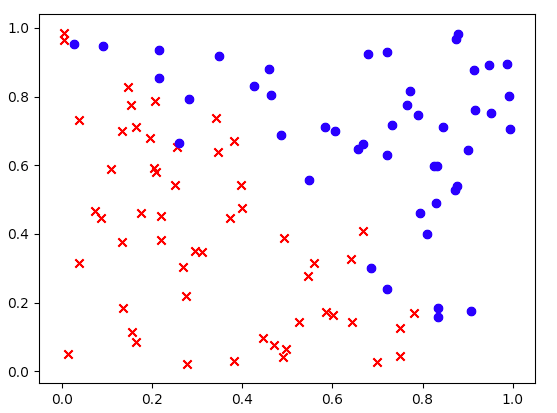
\includegraphics[width=\linewidth]{pics/F1b-b.png}
    \caption{Dataset A}\label{fig:dataset-a}
\end{subfigure}
\begin{subfigure}[b]{0.5\linewidth}
    \centering
    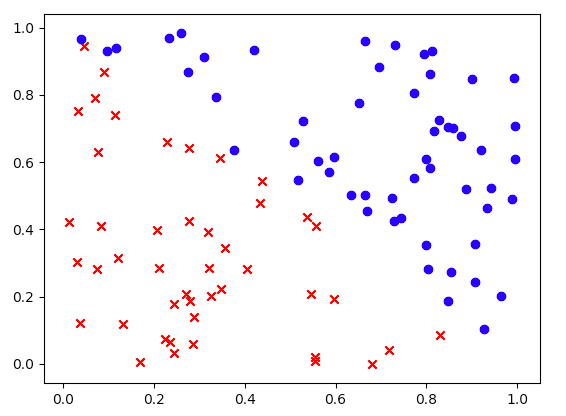
\includegraphics[width=\linewidth]{pics/F1b-a.png}
    \caption{Dataset B}\label{fig:dataset-b}
\end{subfigure}
\caption{Datasets}
\label{fig:datasets}
\end{figure}

Figure~\subref{fig:dataset-a} and Figure~\subref{fig:dataset-b} shows the two datasets. The problem is that dataset B is perfectly linearly separable. 

Consider optimizing objective:

$$
    L(\theta) = \prod_{i=1}^mp(y^{(i)}|x^{(i)};\theta) = \frac{1}{1 + e^{-y^{(i)}\theta^T x^{(i)}}}
$$

    If the dataset is linearly seperable, then for some optimal $\theta$, $y^{(i)}\theta^T x^{(i)}$ will always be positive. In this case, we can multiply $\theta$ by a larger scalar to get larger $L(\theta)$. However, when the dataset is not linearly seperable, this is not the case.


\end{answer}


} \fi


  \item \subquestionpoints{5}
For each of these possible modifications, state whether or not it would lead to
the provided training algorithm converging on datasets such as $B$. Justify your
answers.
\begin{enumerate}
  \item Using a different constant learning rate.
  \item Decreasing the learning rate over time (e.g. scaling the initial
  learning rate by $1/t^2$, where $t$ is the number of gradient descent
  iterations thus far).
  \item Linear scaling of the input features.
  \item Adding a regularization term $\|\theta\|_2^2$ to the loss function.
  \item Adding zero-mean Gaussian noise to the training data or labels.
\end{enumerate}
 
\ifnum\solutions=1 {
  \begin{answer}
\end{answer}

} \fi

 
  
  \item \subquestionpoints{2}
Support vector machines (SVMs) are an alternative machine learning model that we discussed in class.
We have provided you an SVM implementation (using a radial basis function (RBF) kernel) within \texttt{src/svm.py} (You should not need to modify that code).

One important part of training an SVM parameterized by an RBF kernel is choosing an appropriate kernel radius.

Complete the \texttt{compute\_best\_svm\_radius} by writing code to compute the best SVM radius which maximizes accuracy on the validation dataset.

The provided code will use your \texttt{compute\_best\_svm\_radius} to compute and then write the best radius into \texttt{output/p06\_optimal\_radius}.

\ifnum\solutions=1 {
  \begin{answer}
No. SVM's objective is directly associated to geometric margin, which is independent with the scaling of $\theta$.
\end{answer}

} \fi



\end{enumerate}

\textbf{Hint:} Recall the distinction between functional margin and geometric
margin.
